% !Mode:: "TeX:UTF-8"
%!TEX program  = xelatex

\documentclass[bwprint]{gmcmthesis}
%\documentclass{cumcmthesis}
%\documentclass[withoutpreface,bwprint]{cumcmthesis} %去掉封面与编号页,电子版提交的时候使用。

\usepackage[framemethod=TikZ]{mdframed}
\title{全降低汽油精制过程中的辛烷值损失模型}


%参赛信息
\baominghao{20100130029} %参赛队号
\schoolname{北京邮电大学}%学校名称
\membera{唐麒淳} %队员AB
\memberb{段祥卿} %队员B
\memberc{戴维} %队员C


% \usepackage{enumitem}
% \setlist[enumerate]{listparindent=\parindent}
\begin{document}


 %生成标题
 \maketitle


 %填写摘要
\begin{abstract}
摘要文字,请删除我巴拉巴拉


问题一:唐麒淳

问题二:唐麒淳

问题三:唐麒淳

问题四:唐麒淳

问题五:唐麒淳

%填写关键字
\keywords{分布转换\quad 基于模型的特征筛选\quad 贝叶斯优化\quad 5折交叉验证\quad TPE算法}
\end{abstract}

%视情况决定是否需要建立新页面
%\newpage


%设置页码???
\pagestyle{plain}

%目录 不推荐加
%\tableofcontents

%生成目录
\tableofcontents
\newpage


%第一章节
\section{问题重述}
\subsection{问题背景}
巴拉巴拉一堆话
\subsection{问题提出}

\textbf{问题1:巴拉巴拉几个字}

巴拉巴拉一堆话巴拉巴拉一堆话巴拉巴拉一堆话巴拉巴拉一堆话巴拉巴拉一堆话巴拉巴拉一堆话巴拉巴拉一堆话巴拉巴拉一堆话巴拉巴拉一堆话巴拉巴拉一堆话巴拉巴拉一堆话巴拉巴拉一堆话巴拉巴拉一堆话巴拉巴拉一堆话巴拉巴拉一堆话巴拉巴拉一堆话巴拉巴拉一堆话巴拉巴拉一堆话巴拉巴拉一堆话


\textbf{问题2:}

\textbf{问题3:}

\textbf{问题4:}

\textbf{问题5:}


%第二章节
\section{模型假设}

%有序列表 这里写论文的模型假设
%左侧缩进可能还需要调整
\begin{enumerate}[itemindent=20pt]
	\item 假设一
	\item 假设二
\end{enumerate}


%第三章节
\section{符号说明}

\begin{table}[htbp]
    \centering
    \caption{论文中用到的符号定义}
	\begin{tabular}{cc}
	\toprule
	 \makebox[0.4\textwidth][c]{符号}	&  \makebox[0.5\textwidth][c]{意义} \\ 
	 \midrule
	 D	    & 木条宽度(cm)  \\
	 N	    & 第n根木条  \\ 
	   \midrule
	 T	    & 木条根数  \\
	 H	    & 桌子高度(cm)  \\
	 \bottomrule
	\end{tabular}
    \label{tab:addlabel}%
\end{table}%


% \begin{tabular}{cc}
% \toprule
%  \makebox[0.4\textwidth][c]{符号}	&  \makebox[0.5\textwidth][c]{意义} \\ 
%  D	    & 木条宽度(cm)  \\
%  L	    & 木板长度(cm)  \\
%  W	    & 木板宽度(cm)  \\
%  N	    & 第n根木条  \\ 
%    \midrule
%  T	    & 木条根数  \\
%  H	    & 桌子高度(cm)  \\
%  R	    & 桌子半径(cm)  \\
%  R	    & 桌子直径(cm)  \\

%  \bottomrule
% \end{tabular}



%第四章节
\section{问题分析与求解}
\subsection{问题一:巴拉巴拉}
\subsubsection{问题分析}

巴拉巴拉一堆话巴拉巴拉一堆话巴拉巴拉一堆话巴拉巴拉一堆话巴拉巴拉一堆话巴拉巴拉一堆话巴拉巴拉一堆话巴拉巴拉一堆话巴拉巴拉一堆话巴拉巴拉一堆话巴拉巴拉一堆话巴拉巴拉一堆话巴拉巴拉一堆话巴拉巴拉一堆话巴拉巴拉一堆话巴拉巴拉一堆话巴拉巴拉一堆话巴拉巴拉一堆话巴拉巴拉一堆话
\subsubsection{场景建模或者其他}

\subsubsection{特征设计及其他}


\subsection{问题二:巴拉巴拉}
\subsubsection{问题分析}

巴拉巴拉一堆话巴拉巴拉一堆话巴拉巴拉一堆话巴拉巴拉一堆话巴拉巴拉一堆话巴拉巴拉一堆话巴拉巴拉一堆话巴拉巴拉一堆话巴拉巴拉一堆话巴拉巴拉一堆话巴拉巴拉一堆话巴拉巴拉一堆话巴拉巴拉一堆话巴拉巴拉一堆话巴拉巴拉一堆话巴拉巴拉一堆话巴拉巴拉一堆话巴拉巴拉一堆话巴拉巴拉一堆话
\subsubsection{场景建模或者其他}

\subsubsection{特征设计及其他}


\subsection{问题三:巴拉巴拉}
\subsubsection{问题分析}

巴拉巴拉一堆话巴拉巴拉一堆话巴拉巴拉一堆话巴拉巴拉一堆话巴拉巴拉一堆话巴拉巴拉一堆话巴拉巴拉一堆话巴拉巴拉一堆话巴拉巴拉一堆话巴拉巴拉一堆话巴拉巴拉一堆话巴拉巴拉一堆话巴拉巴拉一堆话巴拉巴拉一堆话巴拉巴拉一堆话巴拉巴拉一堆话巴拉巴拉一堆话巴拉巴拉一堆话巴拉巴拉一堆话
\subsubsection{场景建模或者其他}

\subsubsection{特征设计及其他}
\subsection{问题四:巴拉巴拉}
\subsubsection{问题分析}

巴拉巴拉一堆话巴拉巴拉一堆话巴拉巴拉一堆话巴拉巴拉一堆话巴拉巴拉一堆话巴拉巴拉一堆话巴拉巴拉一堆话巴拉巴拉一堆话巴拉巴拉一堆话巴拉巴拉一堆话巴拉巴拉一堆话巴拉巴拉一堆话巴拉巴拉一堆话巴拉巴拉一堆话巴拉巴拉一堆话巴拉巴拉一堆话巴拉巴拉一堆话巴拉巴拉一堆话巴拉巴拉一堆话
\subsubsection{场景建模或者其他}

\subsubsection{特征设计及其他}
\subsection{问题五:巴拉巴拉}
\subsubsection{问题分析}

巴拉巴拉一堆话巴拉巴拉一堆话巴拉巴拉一堆话巴拉巴拉一堆话巴拉巴拉一堆话巴拉巴拉一堆话巴拉巴拉一堆话巴拉巴拉一堆话巴拉巴拉一堆话巴拉巴拉一堆话巴拉巴拉一堆话巴拉巴拉一堆话巴拉巴拉一堆话巴拉巴拉一堆话巴拉巴拉一堆话巴拉巴拉一堆话巴拉巴拉一堆话巴拉巴拉一堆话巴拉巴拉一堆话
\subsubsection{场景建模或者其他}

\subsubsection{特征设计及其他}


%第五章节
%下面这块看看怎么改
\section{模型评价}


\subsection{模型的优点}
巴拉巴拉一堆话巴拉巴拉一堆话巴拉巴拉一堆话巴拉巴拉一堆话巴拉巴拉一堆话巴拉巴拉一堆话巴拉巴拉一堆话巴拉巴拉一堆话巴拉巴拉一堆话巴拉巴拉一堆话巴拉巴拉一堆话巴拉巴拉一堆话巴拉巴拉一堆话巴拉巴拉一堆话巴拉巴拉一堆话巴拉巴拉一堆话巴拉巴拉一堆话巴拉巴拉一堆话巴拉巴拉一堆话



\subsection{模型的缺点}
巴拉巴拉一堆话巴拉巴拉一堆话巴拉巴拉一堆话巴拉巴拉一堆话巴拉巴拉一堆话巴拉巴拉一堆话巴拉巴拉一堆话巴拉巴拉一堆话巴拉巴拉一堆话巴拉巴拉一堆话巴拉巴拉一堆话巴拉巴拉一堆话巴拉巴拉一堆话巴拉巴拉一堆话巴拉巴拉一堆话巴拉巴拉一堆话巴拉巴拉一堆话巴拉巴拉一堆话巴拉巴拉一堆话






\section{加图的方法,记得删除}
\begin{figure}[!h]
\centering
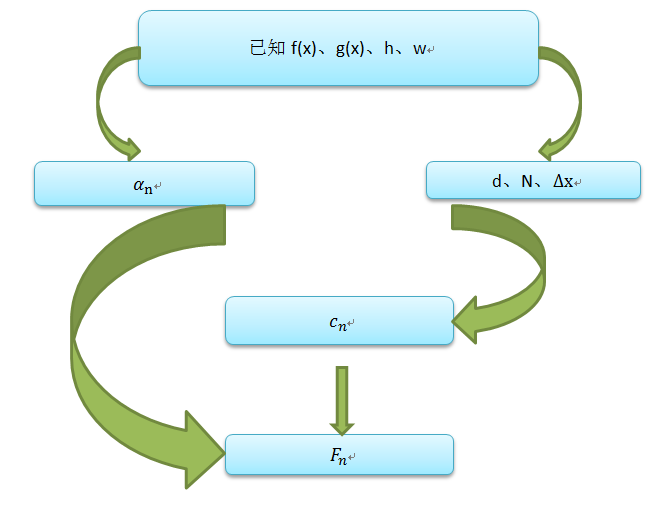
\includegraphics[width=.7\textwidth]{1.png}
\caption{问题三流程图}
\end{figure}



%下面两种参考文献的格式二选一

%参考文献重新分页
\newpage

% 参考文献   手工录入
% \begin{thebibliography}{9}%宽度9
% \bibitem{bib:one} ....
% \bibitem{bib:two} ....
% \end{thebibliography}


\begin{thebibliography}{99}  
\bibitem{ref1}Zheng L, Wang S, Tian L, et al., Query-adaptive late fusion for image search and person re-identification, Proceedings of the IEEE Conference on Computer Vision and Pattern Recognition, 2015: 1741-1750.  
\bibitem{ref2}Arandjelović R, Zisserman A, Three things everyone should know to improve object retrieval, Computer Vision and Pattern Recognition (CVPR), 2012 IEEE Conference on, IEEE, 2012: 2911-2918.  
\bibitem{ref3}Lowe D G. Distinctive image features from scale-invariant keypoints, International journal of computer vision, 2004, 60(2): 91-110.  
\bibitem{ref4}Philbin J, Chum O, Isard M, et al. Lost in quantization: Improving particular object retrieval in large scale image databases, Computer Vision and Pattern Recognition, 2008. CVPR 2008, IEEE Conference on, IEEE, 2008: 1-8.  
\end{thebibliography}


% %采用bibtex方案
% \cite{mittelbach_latex_2004,wright_latex3_2009,beeton_unicode_2008,vieth_experiences_2009}

% \bibliographystyle{gmcm}
% \bibliography{example}


%参考文献 2019年大学生数学建模比赛的模板中提取的
\begin{thebibliography}{9}%宽度9
    \bibitem{1}{liuhaiyang2013latex}
    刘海洋.
    \newblock \LaTeX {}入门\allowbreak[J].
    \newblock 电子工业出版社, 北京, 2013.
    \bibitem{2}{mathematical-modeling}
    全国大学生数学建模竞赛论文格式规范 (2020 年 8 月 25 日修改).
    \bibitem{3} \url{https://www.latexstudio.net}
\end{thebibliography}






\newpage
%附录
\appendix
%\setcounter{page}{1} %如果需要可以自行重置页码。
\section{我的 Python 源程序}
\begin{lstlisting}[language=Python]%设置不同语言即可。
kk=2;[mdd,ndd]=size(dd);
while ~isempty(V)
[tmpd,j]=min(W(i,V));tmpj=V(j);
for k=2:ndd
[tmp1,jj]=min(dd(1,k)+W(dd(2,k),V));
tmp2=V(jj);tt(k-1,:)=[tmp1,tmp2,jj];
end
tmp=[tmpd,tmpj,j;tt];[tmp3,tmp4]=min(tmp(:,1));
if tmp3==tmpd, ss(1:2,kk)=[i;tmp(tmp4,2)];
else,tmp5=find(ss(:,tmp4)~=0);tmp6=length(tmp5);
if dd(2,tmp4)==ss(tmp6,tmp4)
ss(1:tmp6+1,kk)=[ss(tmp5,tmp4);tmp(tmp4,2)];
else, ss(1:3,kk)=[i;dd(2,tmp4);tmp(tmp4,2)];
end;end
dd=[dd,[tmp3;tmp(tmp4,2)]];V(tmp(tmp4,3))=[];
[mdd,ndd]=size(dd);kk=kk+1;
end; S=ss; D=dd(1,:);


 \end{lstlisting}


\end{document} 